\slajdid{08-s013}
\begin{frame}[label=08-s013]{Održanje naponskih nivoa}
\gusttekst\setlength{\parskip}{4pt}
\begin{columns}[c,onlytextwidth]\column{.27\textwidth}\begin{tikzpicture}[x=1cm,y=1cm,font=\sitneoznake,>=Latex]
\draw(0,0)--(0,3.2);
\foreach\y/\label in{0/0,.25/V_{OL},1/V_{IL},1.95/V_{IH},2.8/V_{OH},3.2/V_{CC}}{\draw(-.12,\y)--(.15,\y);\node[left]at(-.12,\y){$\label$};}
\draw[<->](.13,.25)--(.13,1);\draw[<->](.13,1.95)--(.13,2.8);
\node[align=center,right]at(.32,2.38){Opseg napona\\Logicke jedinice};\node[align=center,right]at(.32,.62){Opseg napona\\Logicke nule};
\end{tikzpicture}

\column{.71\textwidth}
Prilikom povezivanja izlaz jednog logičkog kola biće ulaz u naredno logičko kolo. U većini logičkih familija, logičko kolo nije sposobno da na izlazu za logičku nulu da napon 0V niti za logičku jedinicu napon Vcc. Prema tome za realnu analizu signala u digitalnom sistemu je bitno koji naponi mogu da se u „normalnom“ radu pojave na izlazima, ulazima, u logička kola.\par
$V_{OL}$ (output low) - nominalni napon logičke nule, i predstavlja minimalna napon koje logičko kolo u radnom režim može da postavi na izlaz.\par
$V_{OH}$ (output high) - nominalni napon logičke jedinice, i predstavlja maksimalan napon koje logičko kolo u radnom režimu može postavi na izlaz.
\end{columns}\medskip
\centering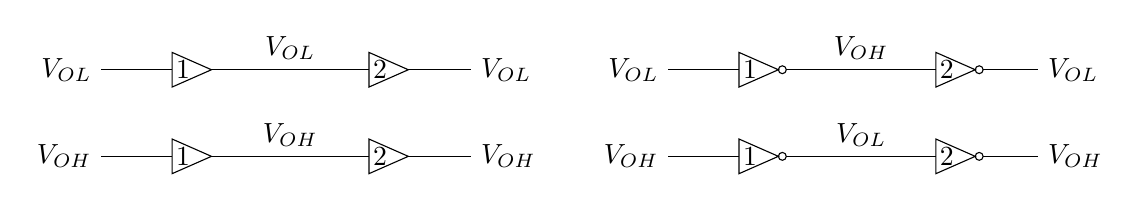
\begin{tikzpicture}[x=1cm,y=1cm,font=\sitneoznake]
\draw(-0.2,0.22)--(0.3,0)--(-0.2,-0.22)--cycle;\node at(-0.06,0){1};
\draw(2.3,0.22)--(2.8,0)--(2.3,-0.22)--cycle;\node at(2.44,0){2};
\draw(-1.1,0)node[left]{$V_{OL}$}--(-0.2,0);
\draw(0.3,0)--(2.3,0)node[midway,above]{$V_{OL}$};
\draw(2.8,0)--(3.6,0)node[right]{$V_{OL}$};
\draw(-0.2,-0.8800000000000001)--(0.3,-1.1)--(-0.2,-1.32)--cycle;\node at(-0.06,-1.1){1};
\draw(2.3,-0.8800000000000001)--(2.8,-1.1)--(2.3,-1.32)--cycle;\node at(2.44,-1.1){2};
\draw(-1.1,-1.1)node[left]{$V_{OH}$}--(-0.2,-1.1);
\draw(0.3,-1.1)--(2.3,-1.1)node[midway,above]{$V_{OH}$};
\draw(2.8,-1.1)--(3.6,-1.1)node[right]{$V_{OH}$};
\draw(7.0,0.22)--(7.5,0)--(7.0,-0.22)--cycle;\node at(7.140000000000001,0){1};
\draw(7.55,0)circle(.05);
\draw(9.5,0.22)--(10.0,0)--(9.5,-0.22)--cycle;\node at(9.639999999999999,0){2};
\draw(10.049999999999999,0)circle(.05);
\draw(6.1,0)node[left]{$V_{OL}$}--(7.0,0);
\draw(7.6000000000000005,0)--(9.5,0)node[midway,above]{$V_{OH}$};
\draw(10.1,0)--(10.8,0)node[right]{$V_{OL}$};
\draw(7.0,-0.8800000000000001)--(7.5,-1.1)--(7.0,-1.32)--cycle;\node at(7.140000000000001,-1.1){1};
\draw(7.55,-1.1)circle(.05);
\draw(9.5,-0.8800000000000001)--(10.0,-1.1)--(9.5,-1.32)--cycle;\node at(9.639999999999999,-1.1){2};
\draw(10.049999999999999,-1.1)circle(.05);
\draw(6.1,-1.1)node[left]{$V_{OH}$}--(7.0,-1.1);
\draw(7.6000000000000005,-1.1)--(9.5,-1.1)node[midway,above]{$V_{OL}$};
\draw(10.1,-1.1)--(10.8,-1.1)node[right]{$V_{OH}$};
\end{tikzpicture}

\end{frame}
